\documentclass{article}
\usepackage[utf8]{inputenc}
\usepackage[english, russian, shorthands=off]{babel}
\usepackage{amsmath,amsfonts,amssymb}
\usepackage{mathtext}
\usepackage[T2A]{fontenc}

%place for text on the page
\usepackage[left=20mm, top=30mm, right=20mm, bottom=30mm, nohead]{geometry}

%Для ссылок
\usepackage{hyperref}
\hypersetup{
	colorlinks=true,
	linkcolor=blue,
	filecolor=magenta,      
	urlcolor=green,
}

% Для картинок
\usepackage{graphicx}
\graphicspath{{pictures/}}
\DeclareGraphicsExtensions{.pdf,.png,.jpg}

% Для рисования в Tikz
\usepackage{pgf,tikz}

% Tikz library for matrix
\usetikzlibrary{matrix}

\usepackage{skak}

% d in the integral
\newcommand{\ud}{\mathrm{d}}

% Для О-большого
\renewcommand{\O}{\mathcal{O}}

% bold symbols qickly
\newcommand{\tb}{\boldsymbol}

% increase vertical space in math-align
\newcommand{\s}{&\\[12pt]}

\usepackage{listings}
\usepackage{xcolor}
\colorlet{punct}{red!60!black}
\definecolor{background}{HTML}{EEEEEE}
\definecolor{delim}{RGB}{20,105,176}
\colorlet{numb}{magenta!60!black}
\lstdefinelanguage{json}{
	basicstyle=\normalfont\ttfamily,
	numbers=left,
	numberstyle=\scriptsize,
	stepnumber=1,
	numbersep=8pt,
	showstringspaces=false,
	breaklines=true,
	frame=lines,
	backgroundcolor=\color{background},
	literate=
	*{0}{{{\color{numb}0}}}{1}
	{1}{{{\color{numb}1}}}{1}
	{2}{{{\color{numb}2}}}{1}
	{3}{{{\color{numb}3}}}{1}
	{4}{{{\color{numb}4}}}{1}
	{5}{{{\color{numb}5}}}{1}
	{6}{{{\color{numb}6}}}{1}
	{7}{{{\color{numb}7}}}{1}
	{8}{{{\color{numb}8}}}{1}
	{9}{{{\color{numb}9}}}{1}
	{:}{{{\color{punct}{:}}}}{1}
	{,}{{{\color{punct}{,}}}}{1}
	{\{}{{{\color{delim}{\{}}}}{1}
	{\}}{{{\color{delim}{\}}}}}{1}
	{[}{{{\color{delim}{[}}}}{1}
	{]}{{{\color{delim}{]}}}}{1},
}

%to fix picture (for [H])
\usepackage{float}

\title{Homework №3}
\author{Вадим Шабашов}
\date{}

\begin{document}
	
	\maketitle
	
	\section*{Задание 1}

\begin{figure}[H]
		\center{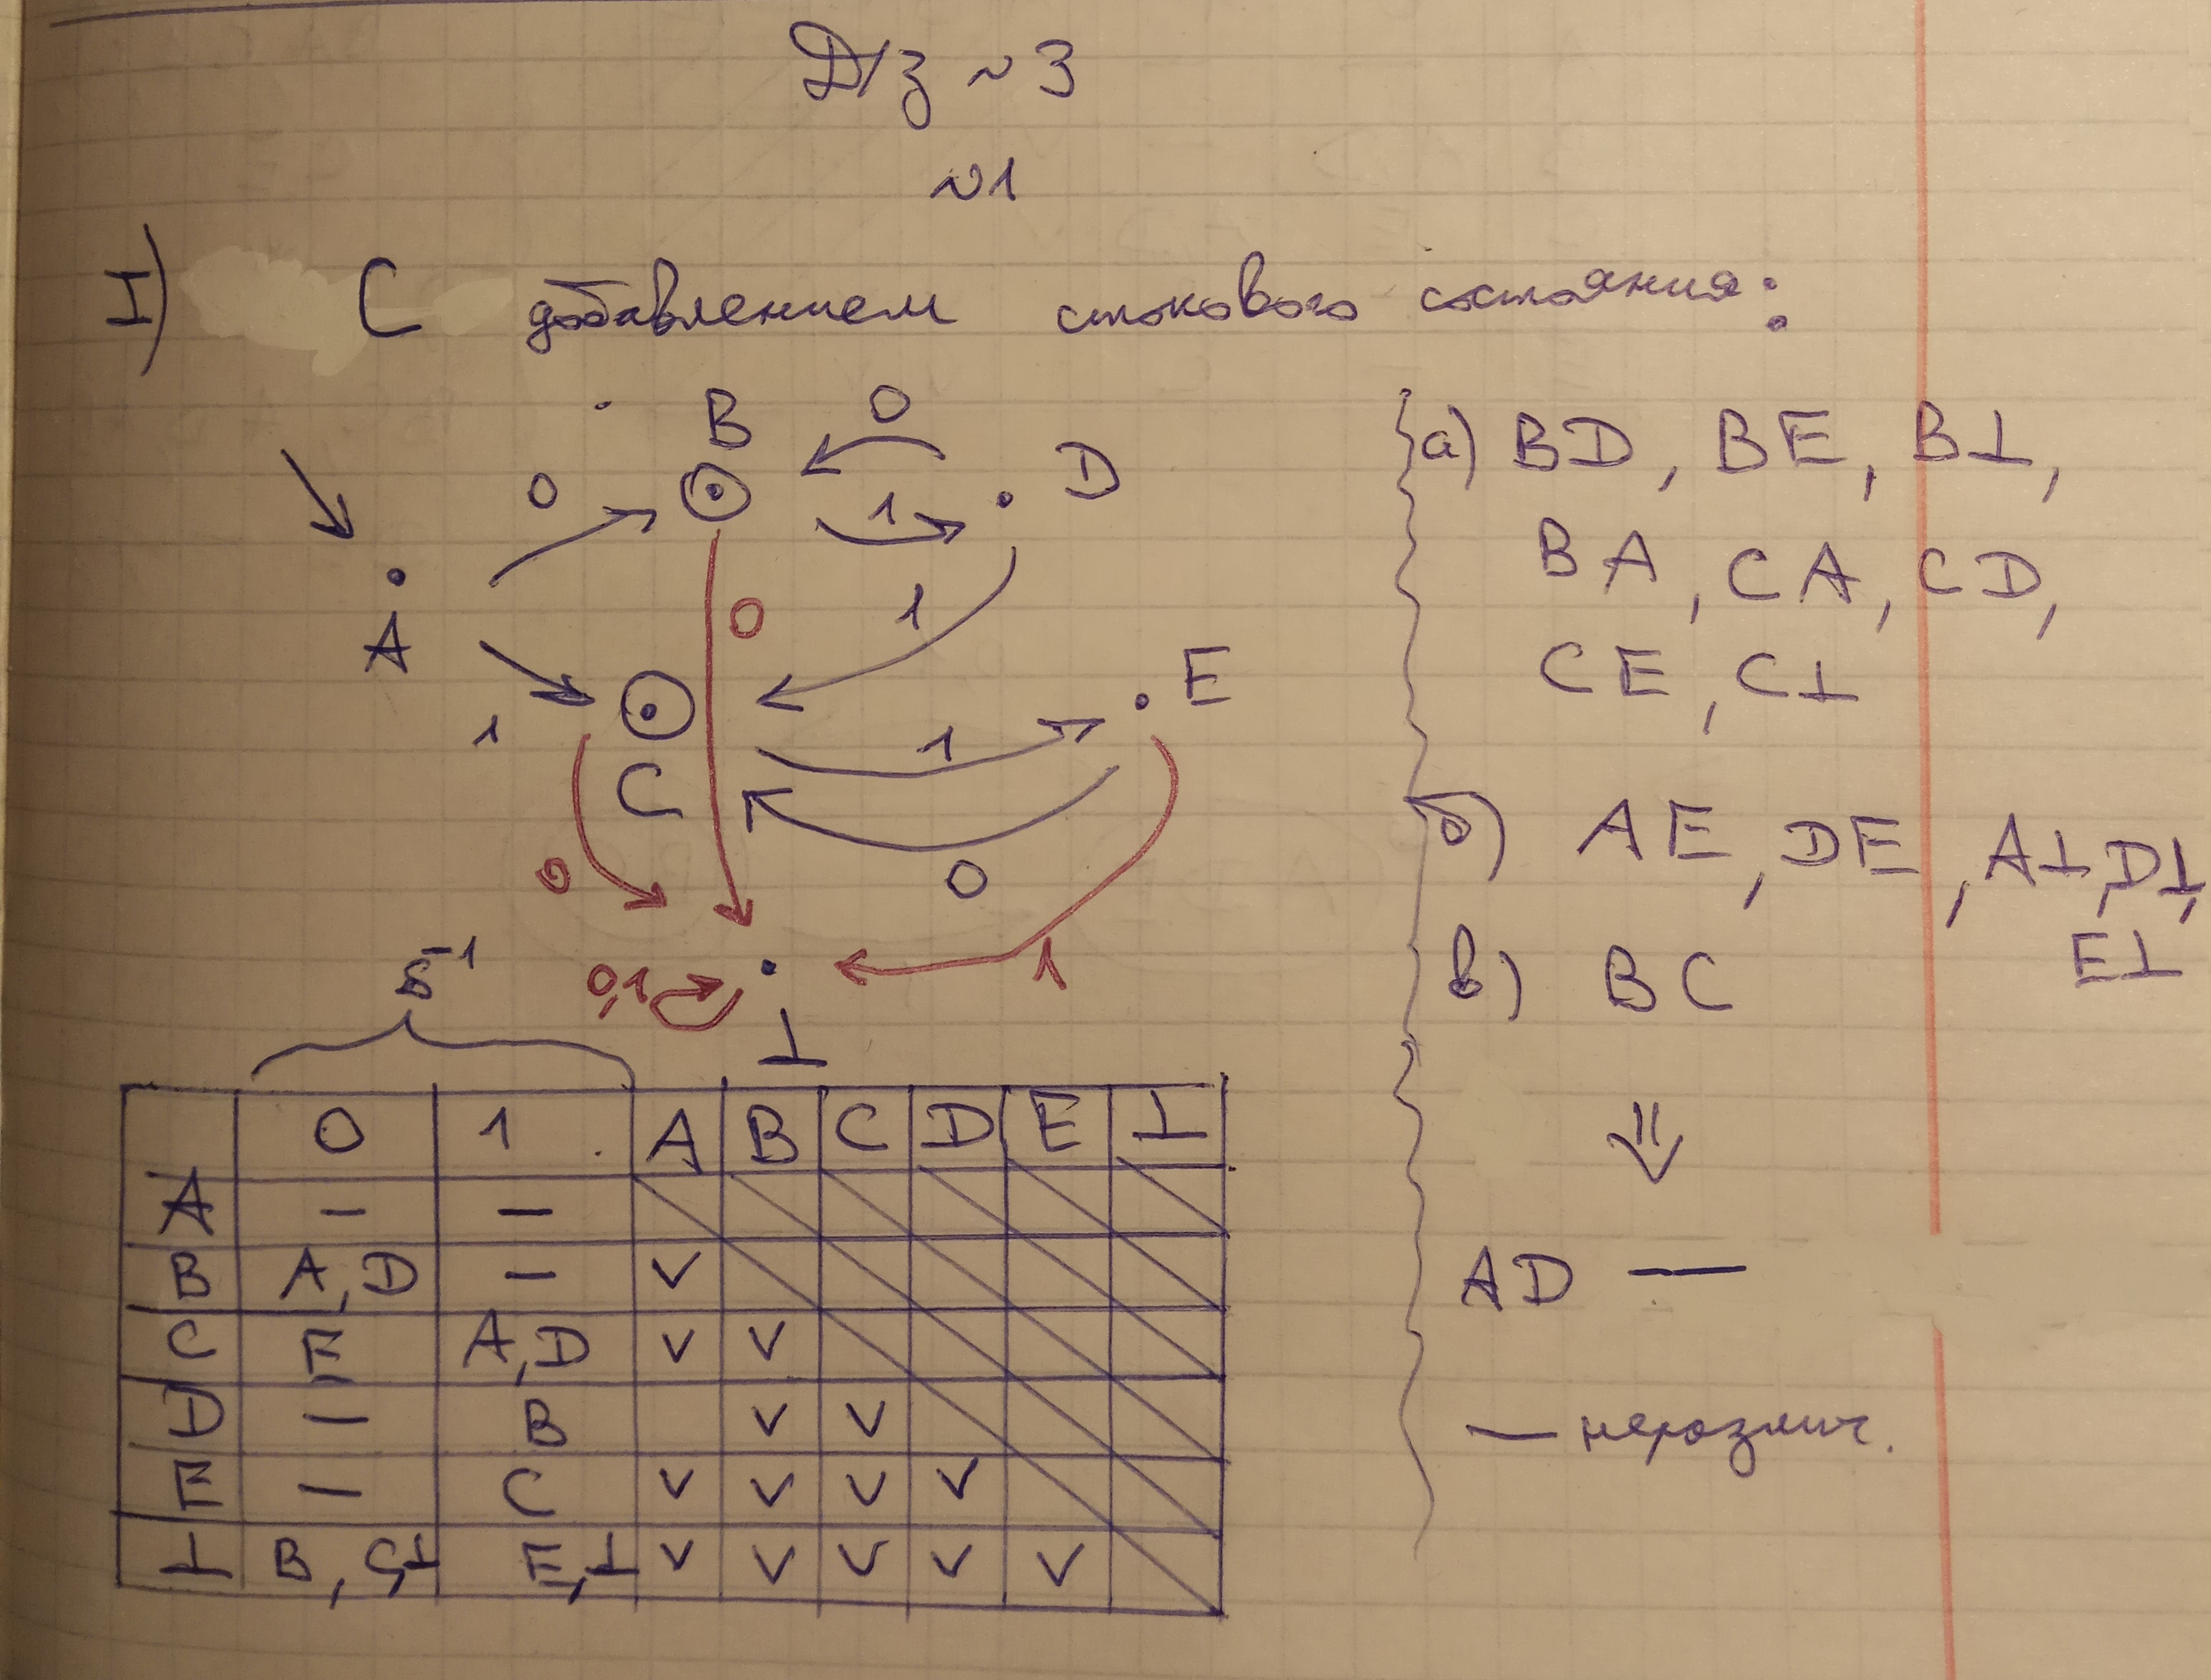
\includegraphics[width=1\linewidth]{1}}
	\end{figure}

\begin{figure}[H]
	\center{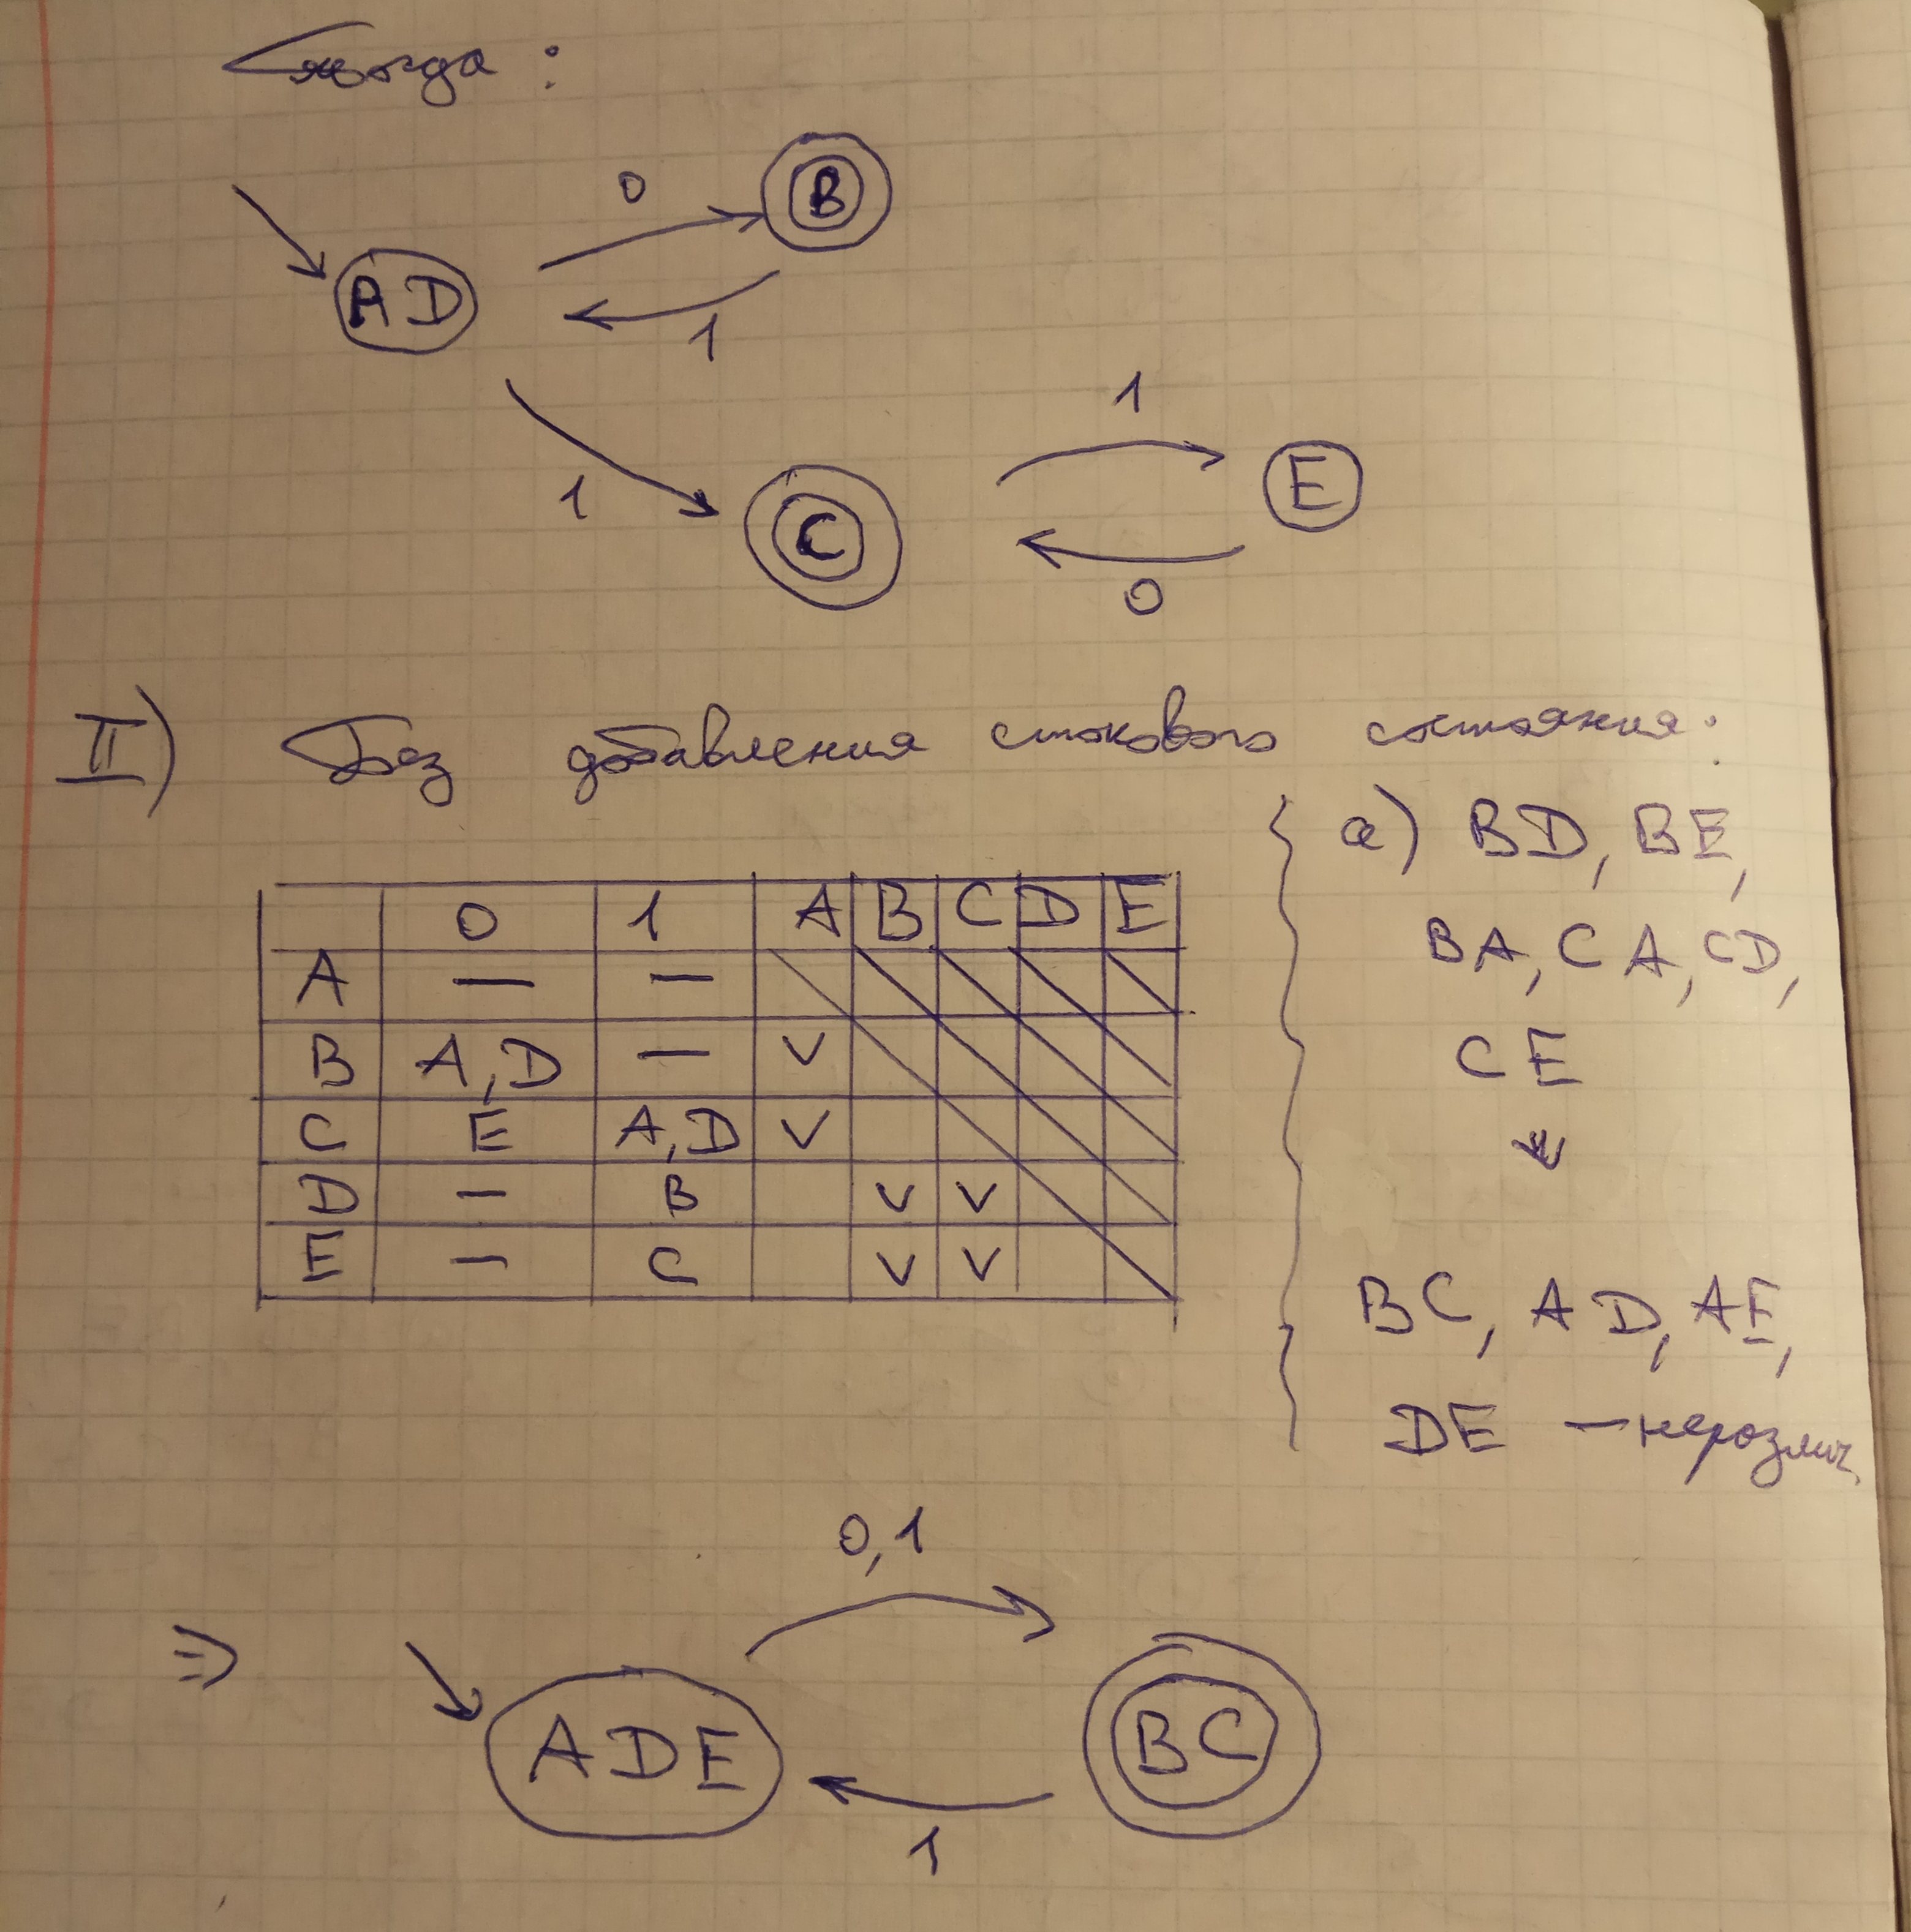
\includegraphics[width=1\linewidth]{2}}
\end{figure}


	\section*{Задание 2}

\begin{enumerate}
	\item Я решил писать конечный автомат на питоне, т.к. знаю этот язык лучше всего. В нем довольно много библиотек для парсинга. В частности библиотека \textrm{json}, которую и решил использовать. Мне показалось, что так будет наибольшая читаемость у формата. Также формат известный, и каждый сможет разобраться, как все храниться очень быстро. Наконец библиотека имеет большую функциональность, поэтому без проблем может парсить сразу "из коробки".
	
	\item Для представления конечного автомата в файле предлагаю использовать следующий вид:
		
\begin{lstlisting}[language=json,firstnumber=1]
{
  "glossary": ["0", "1"],
  "states": ["A", "B", "C", "D", "E"],
  "initial_state": "A",
  "terminal_states": ["B", "C"],
  "edges": [["A", "C", "1"], ["A", "B", "0"], 
  	   ["B", "D", "1"], ["C", "E", "1"], 
  	   ["D", "B", "0"], ["D", "C", "1"], 
  	   ["E", "C", "0"]]
}
\end{lstlisting}

\begin{itemize}
	\item В "glossary" перечисляем алфавит.
	
	\item В "states" перечисляем имена состояний.
	
	\item В "initial\_state" указываем начальное состояние.
	
	\item В "terminal\_states" перечисляем все терминальные состояния.
	
	\item В "edges" перечисляем все ребра. Каждое ребро имеет вид \textrm{[$s_1$, $s_2$, $a$]}, где $s_1, s_2 \in $ "states", $a \in $ "glossary".
\end{itemize}
\end{enumerate}



% \section*{Исправления и доделки}

	
\end{document}
